\documentclass[12pt,a4paper,fleqn]{article}
\usepackage[utf8]{inputenc}
\usepackage[russian]{babel}
\usepackage{amssymb, amsmath, multicol}
\usepackage{enumitem}
\usepackage{lipsum}
\usepackage{euler}
\oddsidemargin=-15.4mm
\textwidth=190mm
\headheight=-32.4mm
\textheight=277mm
\parindent=0pt
\parskip=8pt
\pagestyle{empty}
\usepackage{graphicx}
\begin{document}
\begin{center}
\textbf{\LARGE{Исследовательская работа по теме:\\Исследование функции дифференциальными методами}}\end{center}\newpage\textbf{\LARGE Глава I. Функция}

\begin{center}
$y = $$2^{((82980+1)-0)}$

\end{center}
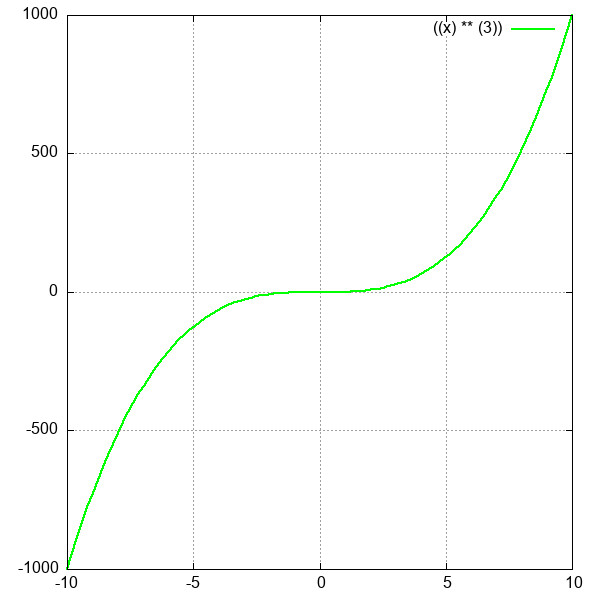
\includegraphics{GraphicDumps/plot.jpg}\newpage \textbf{\LARGE Глава II. Визуальный анализ функции}

//TODO: Лёша, придумай переход. У меня идеи закончились

\begin{center}
$y = $$2^{((82980+1)-0)}$

\end{center}
\newpage \textbf{\LAGRE Глава III. Дифференцирование}

Очевидно, что

\begin{center}
 ($2^{((82980+1)-0)})'
  = 0$\end{center}
\newpage \textbf{\LARGE Глава IV.Упрощение выражения}

\newpage \textbf{\LARGE Глава V. Полученая производная}

$y = $$2^{((82980+1)-0)}$

$y' = $$0$

\includegraphics{GraphicDumps/plot_1.jpg}
\end{document}